\documentclass[logo,reportComp]{thesis}
\usepackage[cpp,pseudo]{mypackage}

\title{操作系统原理实验报告}
\subtitle{实验六:二状态进程模型}
\school{数据科学与计算机学院}
\author{陈鸿峥}
\classname{17大数据与人工智能}
\stunum{17341015}
\headercontext{操作系统原理实验报告}
% \authorremark{本实验报告用\LaTeX撰写,创建时间:\builddate\today}

\begin{document}

\maketitle

\section{实验目的}
\begin{itemize}
	\item 理解二状态进程模型的工作原理
	\item 深刻理解并实施进程管理,包括创建、切换、调度进程等
	\item 在保证进程正常工作的前提下,不破坏原有的基础设施
\end{itemize}

\section{实验要求}
% 实验目的和实验要求由老师提供实验项目文档中获取
保留原型原有特征的基础上,设计满足下列要求的新原型操作系统:
\begin{itemize}
	\item 在C程序中定义进程表,进程数量为4个。
	\item 内核一次性加载4个用户程序运行时,采用时间片轮转调度进程运行,用户程序的输出各占1/4屏幕区域,信息输出有动感,以便观察程序是否在执行。
	\item 在原型中保证原有的系统调用服务可用。再编写1个用户程序,展示系统调用服务还能工作。
\end{itemize}

\section{实验环境}
% 包括:硬件或虚拟机配置方法、软件工具与作用、方案的思想、相关原理、程序流程、算法和数据结构、程序关键模块,结合代码与程序中的位置进行解释。不得抄袭,否则按作弊处理。
% 实验方案包括相关基础原理、实验工具和环境、程序流程和算法思想、数据结构与程序模块功能说明,代码文档组成说明等
具体环境选择原因已在实验一报告中说明。
\begin{itemize}
	\item Windows 10系统 + Ubuntu 18.04(LTS)子系统
	\item gcc 7.3.0 + nasm 2.13.02 + GNU ld (Binutils) 2.3.0
    \item GNU Make 4.1
	\item Oracle VM VirtualBox 6.0.6
    \item Bochs 2.6.9
	\item Sublime Text 3 + Visual Studio Code 1.33.1
\end{itemize}

虚拟机配置:内存4M,1.44M虚拟软盘引导,1.44M虚拟硬盘。

\section{实验方案}
% 包括:主要工具安装使用过程及截图结果、程序过程中的操作步骤、测试数据、输入及输出说明、遇到的问题及解决情况、关键功能或操作的截图结果。不得抄袭,否则按作弊处理。
{\Large\textbf{\textcolor{red}{本次实验进入保护模式。}}}

目前保护模式完成的工作如下:
\begin{itemize}
	\item 32位保护模式基础设施支持
	\begin{itemize}
		\item 全局描述符表(GDT)的创建与管理
		\item 中断描述符表(IDT)的创建与管理:其中也包括了异常(exception)的处理
		\item 任务状态段(TSS)的创建与管理
		\item 内核态(ring 0)与用户态(ring 3)的相互切换
	\end{itemize}
	\item 硬件抽象层(HAL)
	\begin{itemize}
		\item 利用集成驱动电子设施(IDE)进行硬盘读入
		\item 可编程中断控制器(PIC)的初始化与使用
		\item 可编程区间计时器(PIT)的初始化与使用
		\item 键盘驱动
	\end{itemize}
	\item 交互界面(shell)
	\begin{itemize}
		\item 使用Video RAM的显示交互界面,支持键盘输入输出
		\item 简易的命令行解释器
	\end{itemize}
	\item 用户程序(均运行在ring 3进行保护)
	\begin{itemize}
		\item 基本标准库的支持,如\verb'stdio'、\verb'string'等
		\item 系统中断调用(0x80)
	\end{itemize}
	\item 进程控制
	\begin{itemize}
		\item 进程控制块(PCB)的创建与管理
		\item 多进程环境下的进程调入与切出
		\item 从磁盘加载程序、创建进程、调度及执行
	\end{itemize}
\end{itemize}

由于保护模式涵盖的内容非常多,下面将尽可能简练又突出重点地叙述。

\subsection{引导程序---由实模式到保护模式}
本部分对应着\verb'bootloader.asm'文件。

在最开始,操作系统只能进入16位的实模式,引导程序的加载与原来实模式的加载相同。
\begin{itemize}
	\item 处理器会搜索可用的存储媒介,如软盘、硬盘、CD等
	\item 检查每个引导盘的有效性:最后一个字必须为\verb'0x55aa'才为有效的引导盘
	\item 如果有效,则第一个扇区,即主引导程序(master boot record, MBR),将会被加载入RAM地址为\verb'0000:7C00'的地方(也就是物理地址\verb'0x07C00',此过程也被称为自举bootstrap)
	\item 通过BIOS跳转到\verb'0x7C00'继续执行
\end{itemize}

在引导程序中调用写好的汇编例程\verb'load_kernel'(调用BIOS \verb'int 13h'中断读软盘),将内核程序加载到\verb'0x7E00'的地方。

接下来我们就需要从\textbf{实模式切换到保护模式}(\verb'switch_to_pm')。
\begin{itemize}
	\item 关中断\verb'cli'
	\item 通过\verb'lgdt'指令加载全局描述表(其含义可见\ref{sub:gdt}节)
	\item 将控制寄存器\verb'cr0'的第0位设置为1(其含义可见\ref{sub:cr}节)
	\item 通过far jump跳转入32位保护模式,此时处在内核代码段\verb'CODE_SEG'
\end{itemize}

通过上面操作即可成功切换到保护模式。
然后重新将所有段地址设置为内核数据段地址\verb'DATA_SEG',同时设置好栈基址\verb'ebp'和栈指针\verb'esp'。

引导程序的最后就可以直接\verb'call'我们的内核入口地址了!
即\verb'kernel_entry.asm'中的\verb'_start'入口。

\subsubsection{寻址方式}
\label{sub:gdt}
保护模式下的寻址方式与实模式有很大的不同。
\begin{itemize}
	\item 实模式:16位的段寄存器内容左移4位(\verb'10h')作为\textbf{段基地址},加上16位\textbf{段内偏移},形成20位的\textbf{物理地址},实现最大寻址空间$1MB=2^{20}B$。如
	\[\text{segment:offset}=1234h:5678h=12340h+5678h=18018h\]
	\item 保护模式:16位的段寄存器存储的是\textbf{段选择符}(selector),通过访问全局描述符表(global descriptor table, GDT)中对应段描述符的内容,可以得到32位\textbf{段基地址},再与\textbf{段内偏移}相加形成32位\textbf{线性地址}\footnote{由于在本实验中还未开启分页模式,故线性地址即为物理地址。}
	\[\text{descriptor:offset}=10h:5678h=gdt(10h)+2567h\]
\end{itemize}

全局描述符表作为保护模式的核心,关系着内存地址的访问与保护,需要十分熟悉。
每个描述符共64位(8B),如图\ref{fig:gdt}所示。
\begin{figure}[H]
\centering
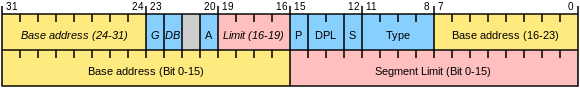
\includegraphics[width=0.8\linewidth]{fig/gdt.png}
\caption{全局描述符表(GDT)}
\label{fig:gdt}
\end{figure}

其中
\begin{itemize}
	\item 0-15、48-51:段界限
	\item 16-39、56-63:基地址
	\item 40-43:描述符类型
	\begin{itemize}
		\item 40:访问位(虚存使用)
		\item 41:0只读(数据段)/只可执行(代码段);1可读可写/可读可执行
		\item 42:扩展方向
		\item 43:0数据段,1代码段
	\end{itemize}
	\item 44:0系统描述符,1代码或数据描述符
	\item 45-46:特权级(ring),0内核态,3用户态,1-2系统态
	\item 47:段是否在内存中(虚存使用)
	\item 52:保留位(OS)
	\item 53:保留位(0)
	\item 54:段类型,0为16位,1为32位
	\item 55:粒度,0无,1界限为4K的倍数
\end{itemize}

我在\verb'gdt.inc'中定义了初始进入保护模式时的三个描述符,按照上面每个位的含义填写并加载
\begin{itemize}
	\item \verb'gdt_null'(0x00):全零描述符
	\item \verb'gdt_code'(0x08):代码段描述符
	\item \verb'gdt_data'(0x10):数据段描述符
\end{itemize}

\subsubsection{控制寄存器}
\label{sub:cr}
x86处理器除了状态寄存器\verb'eflags'、\verb'eip',还有4个32位的控制寄存器,它们都保存着全局与任务无关的机器状态。
\begin{itemize}
	\item \verb'cr0':包含6个预定义标志,其中\textbf{第0位}是我们需要关注的
	\begin{center}
	\begin{tabular}{|c|c|}\hline
	\textbf{标志位} & \textbf{含义}\\\hline
	0(PE) & \textbf{保护模式} \\\hline
	1(MP) & 监控协处理器\\\hline
	2(EM) & 仿真协处理器\\\hline
	3(TS) & 任务切换\\\hline
	4(ET) & 协处理器类型(80287/80387)\\\hline
	5 & 未用\\\hline
	6(PG) & 内存分页\\\hline
	\end{tabular}
	\end{center}
	\item \verb'cr1':未定义的控制寄存器,未来使用
	\item \verb'cr2':页故障线性地址寄存器,保存最后一次出现页故障的全32位线性地址
	\item \verb'cr3':页目录基址寄存器,保存页目录表的物理地址
\end{itemize}

\subsection{硬件抽象层}
硬件抽象层(Hardware Abstraction Layer, HAL)通过将底层的硬件设施进行封装,而只留下上层的API接口,使得通过C语言也可以很方便地进行底层操作。

通过汇编入口(\verb'kernel_entry.asm')\footnote{在该汇编入口程序中,还定义了其他基本的设施,方便后面HAL的调用。}进入内核后,直接跳转入C语言编写的内核(\verb'call main')。
由于保护模式下BIOS都无法使用,故进入内核后第一件事则是初始化各种硬件抽象。

\subsubsection{全局描述符表(GDT)}
由于进入了C的内核,原来在\verb'bootloader.asm'中定义的GDT已经无法定位也很难使用,故需要重新建立GDT并加载。

用C的结构体可以使得GDT的定义比较清晰,如\verb'gdt.h'中所示
\begin{lstlisting}
struct gdt_descriptor {

	// bits 0-15 of segment limit
	uint16_t		limit;

	// bits 0-23 of base address
	uint16_t		baseLo;
	uint8_t			baseMid;

	/*
	 * descriptor access flags
	 * | 7 | 6 | 5 | 4 | 3 | 2 | 1 | 0 |
	 * | P |  DPL  | S |      TYPE     |
	 * P: Present in memory or not
	 * DPL(Descriptor Privilege Level): ring 0 - ring 3
	 * S: 1 - Data/Code descriptor | 0 - gate descriptor
	 * Type: When S = 1
	 *    3: Executable
	 *    2: Consistent
	 *    1: 1 - Read+Write | 0 - Only read
	 *    0: Accessed
	 */
	uint8_t			flags; // access

	/*
	 * grand
	 * | 7 |  6  | 5 |  4  | 3 | 2 | 1 | 0 |
	 * | G | D/B | 0 | AVL |   Limit high  |
	 * G: 0 - B | 1 - 4KB
	 */
	uint8_t			grand; // limit_high, flags

	// bits 24-32 of base address
	uint8_t			baseHi;
} __attribute__((packed));
\end{lstlisting}

注意最后添加\verb'(packed)'的编译指令阻止编译器对该结构体进行对齐优化。
通过下面的API可以方便地设置GDT。
\begin{lstlisting}
void gdt_set_descriptor(uint32_t i, uint64_t base, uint64_t limit, uint8_t access, uint8_t grand)
\end{lstlisting}

初始化以下6个段描述符
\begin{itemize}
	\item \verb'SEG_NULL'(0x00):全零描述符
	\item \verb'SEG_KER_CODE'(0x08):内核代码段描述符
	\item \verb'SEG_KER_DATA'(0x10):内核数据段描述符
	\item \verb'SEG_USER_CODE'(0x18):用户代码段描述符(设置为ring3)
	\item \verb'SEG_USER_DATA'(0x20):用户数据段描述符(设置为ring3)
	\item \verb'SEG_TSS'(0x28):TSS段描述符(见\ref{sub:tss}节)
\end{itemize}

由于重新加载了GDT,故要重新加载入GDT寄存器,其定义如下
\begin{lstlisting}
struct gdtr {

	// size of gdt
	uint16_t		m_limit;

	// base address of gdt
	uint32_t		m_base;
} __attribute__((packed));
\end{lstlisting}

汇编接口\verb'load_gdt'如下,需要重新设置各个段寄存器指向内核代码段,并进行一个\verb'far jump'。
\begin{lstlisting}[language={[x86masm]Assembler}]
[ global load_gdt ]
[ extern _gdtr ]
load_gdt:
	lgdt [ _gdtr ]
	mov ax, 0x10                ; kernel data selector
	mov ds, ax
	mov es, ax
	mov fs, ax
	mov gs, ax
	mov ss, ax
	jmp 0x08:load_gdt_ret
load_gdt_ret:
	ret
\end{lstlisting}

\subsubsection{任务状态段(TSS)}
\label{sub:tss}
保护模式之所以能够保护就是因为它设立了4个不同的特权级
\begin{itemize}
	\item ring0:内核态,权限最高
	\item ring1:系统态
	\item ring2:系统态
	\item ring3:用户态,权限最低
\end{itemize}

当需要从高的特权级向低的特权级转换时,就需要结合任务状态段(Task State Segment, TSS)进行切换。
TSS包含了寄存器、局部描述符表等信息,如下所示。
\begin{lstlisting}
struct tss_entry {
	uint32_t prevTss;
	uint32_t esp0;
	uint32_t ss0;
	uint32_t esp1;
	uint32_t ss1;
	uint32_t esp2;
	uint32_t ss2;
	uint32_t cr3;
	uint32_t eip;
	uint32_t eflags;
	uint32_t eax;
	uint32_t ecx;
	uint32_t edx;
	uint32_t ebx;
	uint32_t esp;
	uint32_t ebp;
	uint32_t esi;
	uint32_t edi;
	uint32_t es;
	uint32_t cs;
	uint32_t ss;
	uint32_t ds;
	uint32_t fs;
	uint32_t gs;
	uint32_t ldt;
	uint16_t trap;
	uint16_t iomap;
} __attribute__((packed));
\end{lstlisting}

在GDT中定义了TSS的入口后,还需通过\verb'ltr'将其加载入寄存器(\verb'tss.h'中定义)。

\subsubsection{中断描述符表(IDT)}
实模式中我们采用中断向量表(Interrupt Vector Table, IVT)给出中断处理程序的入口。
而在保护模式中我们则采用中断描述符表(Interrupt Description Table, IDT)给出中断处理程序的入口。

图\ref{fig:idt}从Intel Developer's Manual Volume 3, Chapter 6中截取。
如果DPL被设置为3,则该中断可以在用户态中被\verb'int'调用。
\begin{figure}[H]
\centering
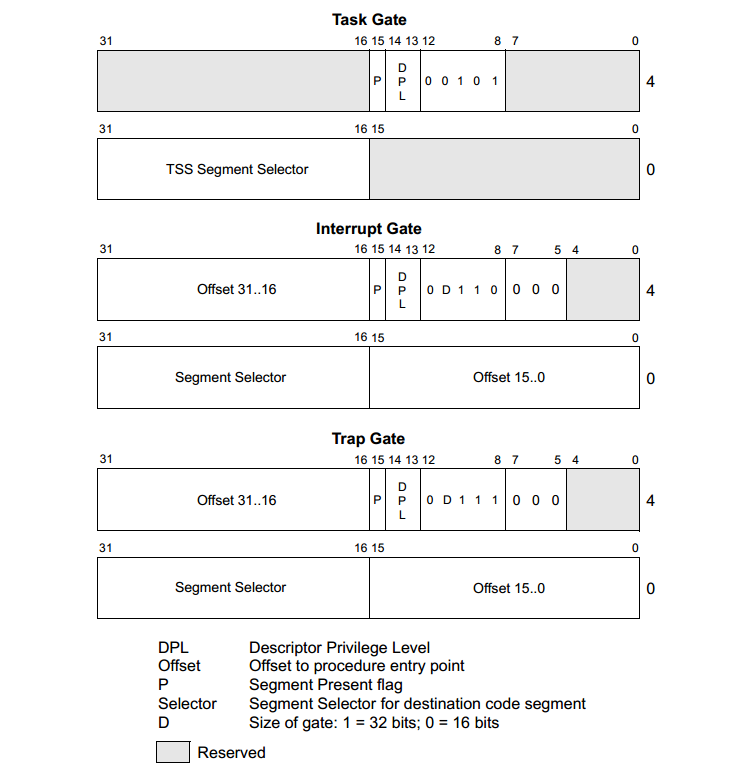
\includegraphics[width=0.7\linewidth]{fig/idt.PNG}
\caption{中断描述符表(IDT)}
\label{fig:idt}
\end{figure}

对应的,可以给出C的结构体
\begin{lstlisting}
struct IDT_entry {
	unsigned short int offset_lowerbits;
	unsigned short int selector;
	unsigned char zero;
	unsigned char type_attr;
	unsigned short int offset_higherbits;
};
\end{lstlisting}

同时给出API接口
\begin{lstlisting}
int install_ir (uint32_t i, uint16_t type_attr, uint16_t selector, uint64_t irq)
void setvect (int intno, uint64_t vect)
\end{lstlisting}

类似于GDT,IDT也有自己的寄存器,需要在初始化时进行加载。
\begin{lstlisting}[language={[x86masm]Assembler}]
; extern void load_idt(unsigned long *idt_ptr); // C function
[ global load_idt ]
load_idt:
	mov edx, [ esp + 4 ]
	lidt [ edx ]        ; load interrupt description table (IDT)
	sti                 ; turn on interrupts
	ret
\end{lstlisting}

加载完IDT后就可以对一些常用的中断号进行设置。
由于是面向x86处理器的操作系统,故采用Intel CPU给出的中断号,如图\ref{fig:exceptions}所示。
\begin{figure}[H]
\centering
\begin{tabular}{c}
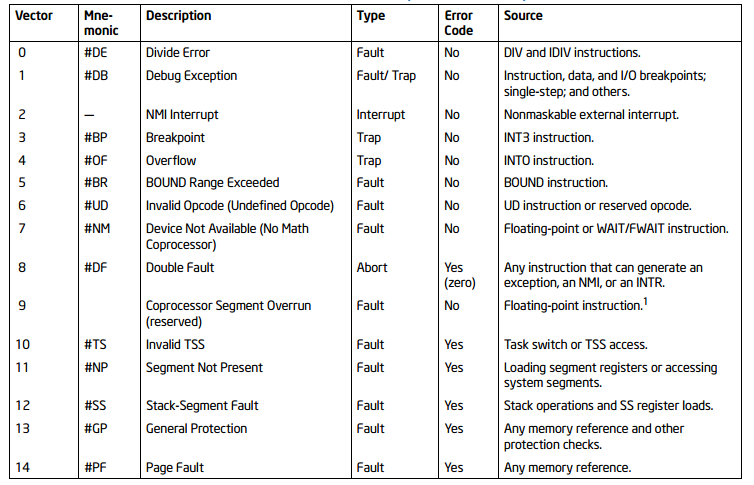
\includegraphics[width=0.8\linewidth]{fig/exceptions1.PNG}\\
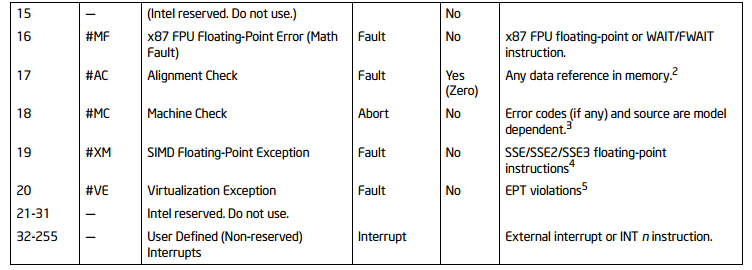
\includegraphics[width=0.8\linewidth]{fig/exceptions2.PNG}
\end{tabular}
\caption{Intel CPU异常中断号}
\label{fig:exceptions}
\end{figure}

在本操作系统中,没有对这些异常进行特别的处理,只是将出错的信息输出,并陷入死循环(见\verb'exception.h')。
对于没有处理的异常,则调用默认中断处理程序,如下。
\begin{lstlisting}
void default_handler () {
	put_error("Error: Unhandled Exception!");
	for(;;);
}
\end{lstlisting}

同时类似Linux将\verb'0x80'设置为系统调用,供用户程序调用。

\subsubsection{可编程中断控制器(PIC)}
8259A微控制器(microcontroller)/可编程中断控制器(Programmable Interrupt Controller, PIC)是CPU与外围设备交互的一个界面。
通过提供中断处理例程(Interrupt Routine, IR),我们就可以处理8259A发出的中断请求(Interrupt Request, IRQ)。

通过\verb'int'指令调用的称为软件中断,而8259A产生的则是硬件中断,如图\ref{fig:hardware_interrupt}所示。
\begin{figure}[H]
\centering
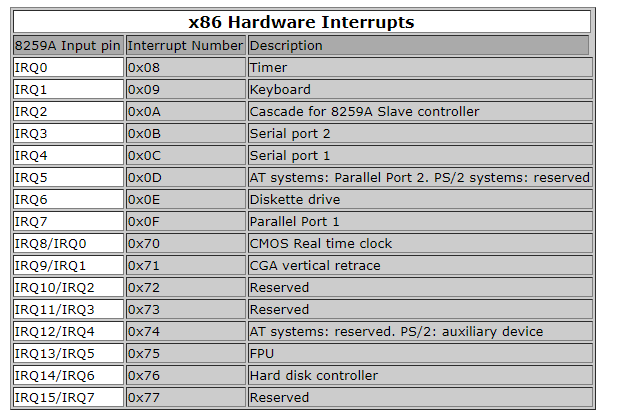
\includegraphics[width=0.8\linewidth]{fig/hardware_interrupt.PNG}
\caption{8259A中断号}
\label{fig:hardware_interrupt}
\end{figure}

处理器都会有自己内部的PIC微处理器,而每一个PIC只支持8个IRQ,因此大多主板(motherboard)都会包含一个二级(secondary)/从(slave)PIC微控制器。
故现在大多计算机都有2个PIC,其连接方式如图\ref{fig:8259A}所示。
\begin{figure}[H]
\centering
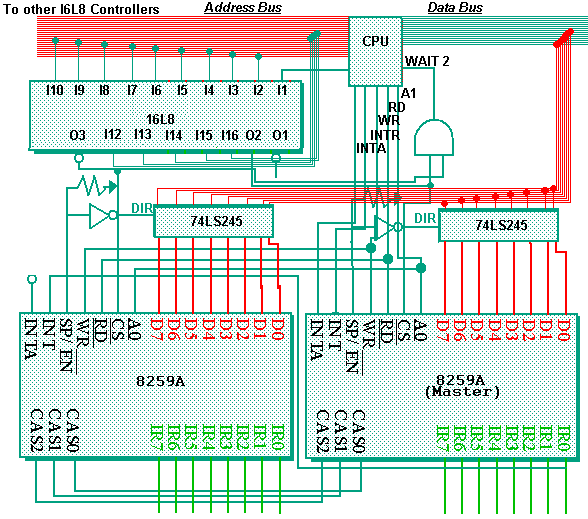
\includegraphics[width=0.6\linewidth]{fig/8259A.png}
\caption{8259A连接方式}
\label{fig:8259A}
\end{figure}

在\verb'pic.h'中,我们可以将这些端口号进行抽象,更加方便编写程序。
\begin{lstlisting}
// The following devices use PIC 1 to generate interrupts
#define		PIC_IRQ_TIMER			0 // IMPORTANT!
#define		PIC_IRQ_KEYBOARD		1 // IMPORTANT!
#define		PIC_IRQ_SERIAL2			3
#define		PIC_IRQ_SERIAL1			4
#define		PIC_IRQ_PARALLEL2		5
#define		PIC_IRQ_DISKETTE		6 // IMPORTANT!
#define		PIC_IRQ_PARALLEL1		7

// The following devices use PIC 2 to generate interrupts
#define		PIC_IRQ_CMOSTIMER		0
#define		PIC_IRQ_CGARETRACE		1
#define		PIC_IRQ_AUXILIARY		4
#define		PIC_IRQ_FPU				5
#define		PIC_IRQ_HDC				6
\end{lstlisting}

通过I/O端口编程,可以实现CPU和8259A的交互。
我们同样可以提供一组I/O指令方便C程序调用,定义在\verb'io.h'中。
\begin{lstlisting}
static inline unsigned char port_byte_in(unsigned short port){
	unsigned char result;
	__asm__ volatile ("in al, dx"
					 :"=a"(result)
					 :"d"(port)
					 );
	return result;
}

static inline void port_byte_out(unsigned short port, unsigned char data){
	__asm__ volatile ("out dx, al"
					 :
					 :"a"(data), "d"(port)
					 );
}
\end{lstlisting}

而初始化的过程通过一系列的\emph{操作命令}(operation command)实现。
操作命令包括\emph{初始化命令字}(Initialization Command Words, ICW)和\emph{操作命令字}(Operation Command Words, OCW)。

初始化过程需要向8259A发送4组ICW,将重要的端口号(如时钟、键盘等)打开,如下所示。
\begin{lstlisting}
void pic_init () {

	uint8_t		icw	= 0;

	// disable hardware interrupts
	disable ();

	// ICW1: Begin initialization of PIC
	icw = (icw & ~PIC_ICW1_MASK_INIT) | PIC_ICW1_INIT_YES; // 00010000
	icw = (icw & ~PIC_ICW1_MASK_IC4) | PIC_ICW1_IC4_EXPECT; // 00010001

	pic_send_command (icw, 0); // 0x11
	pic_send_command (icw, 1); // 0x11

	// ICW2: remap offset address of IDT
	pic_send_data (0x20, 0); // master
	pic_send_data (0x28, 1); // slave

	// ICW3 for master PIC is the IR that connects to secondary pic in binary format
	// ICW3 for secondary PIC is the IR that connects to master pic in decimal format
	pic_send_data (0x04, 0);
	pic_send_data (0x02, 1);

	// ICW4: Enables i86 mode
	icw = (icw & ~PIC_ICW4_MASK_UPM) | PIC_ICW4_UPM_86MODE; // 00010001
	pic_send_data (icw, 0);
	pic_send_data (icw, 1);

	enable();
}
\end{lstlisting}

\subsubsection{键盘中断}
由于在PIC初始化中我们已经将主控制器的端口号映射到\verb'0x20'开始的8个中断,故键盘将对应着\verb'0x21'号中断,我们只需要提供键盘中断处理程序\verb'keyboard_handler_main'即可。
而通过I/O端口读入的为按键的扫描码(定义在\verb'scancode.h'),需要将扫描码转化为ASCII码才能为我们使用。
\begin{lstlisting}
void keyboard_handler_main(void)
{
	unsigned char status;
	char keycode;

	/* write End of Interrupt (EOI) */
	port_byte_out(0x20, 0x20);

	status = port_byte_in(KEYBOARD_STATUS_PORT);
	/* Lowest bit of status will be set if buffer is not empty */
	if (status & 0x01) {
		keycode = port_byte_in(KEYBOARD_DATA_PORT);
		if (keycode < 0)
			return;

		char ascii = asccode[(unsigned char) keycode][0];
		kb_char = ascii;
	}
}
\end{lstlisting}

每次检测到按键就将当前按键的扫描码转化为ASCII码,然后存入缓冲区\verb'kb_char'中,结束中断。
同时,我们可以提供一个API,即\verb'getchar()',检测缓冲区的内容是否合法,若合法则将其内容取出来返回,如下所示。
\begin{lstlisting}
char getchar()
{
	char c = INVALID_KB_CHAR;
	kb_char = INVALID_KB_CHAR;
	while (c == INVALID_KB_CHAR)
		c = kb_char;
	kb_char = INVALID_KB_CHAR;
	return c;
}
\end{lstlisting}

由于中断处理需要采用\verb'iret'返回,故实现时都提供了汇编入口,然后调用C的处理程序进行中断处理。
注意在中断处理时应先关中断,然后再打开,如下面的例子所示。
\begin{lstlisting}[language={[x86masm]Assembler}]
; setvect(0x21,(unsigned long)keyboard_handler); // keyboard uses #33 interrupt
keyboard_handler:
	cli
	call    keyboard_handler_main ; C function
	sti
	iretd                         ; 32-bit return
\end{lstlisting}

有\verb'getchar()'函数后,就可以实现C的标准库\verb'stdio.h'。常用的函数均已实现,如下
\begin{itemize}
	\item \verb'getchar'、\verb'getline'
	\item \verb'scanf'、\verb'sscanf'
	\item \verb'printf'
	\item \verb'put_error'、\verb'put_info'
	\item \verb'clear_screen'
\end{itemize}
其他更细的函数请直接查看源程序。
光标的处理与前几次实验相同,在此不再赘述。

\subsubsection{可编程区间计时器(PIT)}
可编程区间计时器(Programmable Interval Timer, PIT)是处理器内置的时间计数器,每进行一次计数就会触发中断,需要处理器进行处理。
通过下面的API可以创建一个计时器,同时将频率设置为100Hz。
\begin{lstlisting}
void pit_start_counter (uint32_t freq, uint8_t counter, uint8_t mode)
\end{lstlisting}

有了PIC的铺垫,PIT的编程就方便很多。
类似于键盘的初始化,只需设置中断号和中断处理程序即可。
\begin{lstlisting}
setvect (32, (unsigned long)pit_handler); // pit uses #32 interrupt
\end{lstlisting}

由于时间中断处理对于分时操作系统有着至关重要的作用,其涉及到进程的切换,故在\ref{sub:process}节才进行阐述。

\subsubsection{磁盘控制}
由于BIOS被禁用了,故从磁盘读取数据依然要自己进行编程。
本来想通过直接编写软盘驱动来读取数据,但尝试了多次都无法成功。
后来迫不得已使用集成驱动电子设备(Integrated Drive Electronics, IDE)进行读取,缺点是需要新建一个虚拟硬盘并挂载入虚拟机,但好处是编程十分方便。

如下所示,直接传入要读的磁盘扇区号,即可通过以下几条指令对IDE/ATA端口进行编程,一次性将扇区读取出来。
\begin{lstlisting}
/* readsect - read a single sector at @secno into @dst */
static void readsect(uintptr_t dst, uint32_t secno) {

    port_byte_out(0x1F2, 1);                         // count = 1
    port_byte_out(0x1F3, secno & 0xFF);
    port_byte_out(0x1F4, (secno >> 8) & 0xFF);
    port_byte_out(0x1F5, (secno >> 16) & 0xFF);
    port_byte_out(0x1F6, ((secno >> 24) & 0xF) | 0xE0);
    port_byte_out(0x1F7, 0x20);                      // cmd 0x20 - read sectors
    // wait for disk to be ready
    waitdisk();

    // read a sector
    insw(0x1F0, dst, SECTSIZE / 2);
}
\end{lstlisting}

其中,\verb'insw'函数对应着x86汇编的\verb'rep insw'指令,可以一次性将字符串从I/O端口缓冲区中读入对应内存地址。

这里类似于1.44M软盘的格式创建了一个同样是1.44M的虚拟硬盘(2磁头、80磁道、每道18扇区)。

\subsubsection{其他API}
硬件抽象层还提供了其他API,如下
\begin{itemize}
	\item \verb'generate_interrupt':生成中断
	\item \verb'sleep':使用PIT的计数器计数,超过指定时间才退出,进而实现等待的功能
\end{itemize}

\subsection{堆栈}
由于堆栈在操作系统实验中非常重要,故单独开一节阐述。

\subsubsection{函数调用}
由于操作系统内核采用C和汇编混编,故函数调用有两种情况,重点需要考虑如何利用堆栈传递函数参数。

\begin{enumerate}
\item 汇编调用C函数:通过\verb'push'将参数依次进栈,然后直接\verb'call'调用C中对应函数。
而C函数的参数列表从左到右依次从栈顶中读出。
样例如下
\begin{lstlisting}[language={[x86masm]Assembler}]
[ extern test_function ]
push arg2
push arg1
call test_function
; void test_function(int arg1, int arg2); // C function
\end{lstlisting}

\item C函数调用汇编:函数参数从右往左入栈,在汇编中则由右往左弹出。
通过加\\\verb'__attribute__((__cdecl__))'编译指令,强制进栈次序,并且可以实现变参数传递。
\begin{lstlisting}
// extern void test_function(int arg1, int arg2); // assembly
test_function(arg1, arg2); // directly call
// pop eax ; arg1
// pop ebx ; arg2
\end{lstlisting}
\end{enumerate}

在保护模式中,由于存在不同的段选择子,故\verb'call'和\verb'ret'都有远(far)和近(near)之分。
在相同段内的调用/返回则是近的,在不同段间的调用/返回则是远的。
其堆栈内容如图\ref{fig:call_stack}\footnote{Intel Manual Volume 1, Chapter 6, Procedure Calls, Interrupts, and Exceptions}所示。
\begin{figure}[H]
\centering
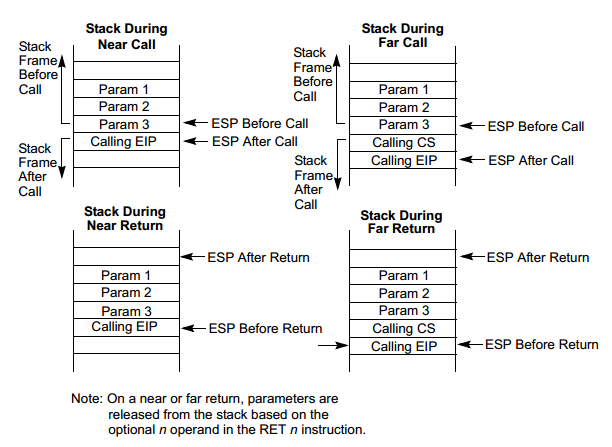
\includegraphics[width=0.7\linewidth]{fig/call.PNG}
\caption{函数调用堆栈}
\label{fig:call_stack}
\end{figure}

\subsubsection{硬件中断与返回}
这一节的内容同样很关键,是后面做进程切换的核心。

当产生中断/异常时,硬件会自动将\verb'eflags'、\verb'cs'和\verb'eip'进行堆栈,至于有没有\verb'error code'则要看情况。
但对于保护模式来说,由于涉及特权级的切换,所以问题会多很多。
如图\ref{fig:interrupt-stack}\footnote{Intel Manual Volume 3, Chapter 6, Interrupt and Exception Handling}所示,当中断处理程序和原程序特权级相同时,使用同一个堆栈。
而特权级不同时,则会发生堆栈切换,参数都会被堆到新的栈中。
同时\verb'ss'和\verb'esp'会作为最开始的元素进入栈中,方便中断处理后的返回。
\begin{figure}[H]
\centering
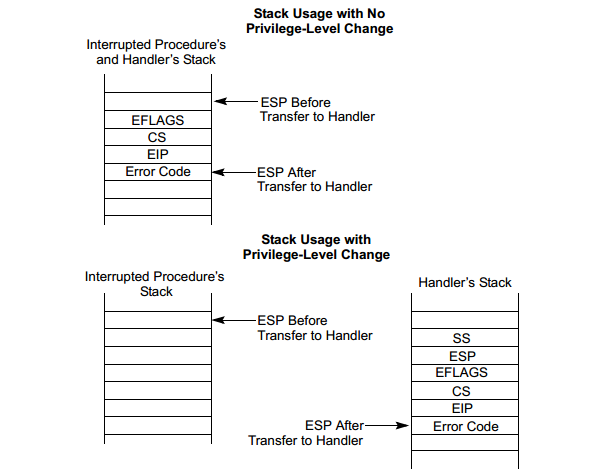
\includegraphics[width=0.7\linewidth]{fig/interrupt-stack.PNG}
\caption{中断堆栈}
\label{fig:interrupt-stack}
\end{figure}

\verb'iret'可谓是保护模式中最重要的一条指令了,它的功能如下
\begin{itemize}
\item 自动从当前栈顶弹出\verb'cs:eip',作为返回地址
\item 设置新的标志位为\verb'eflags'
\item 如果发生特权级切换,还需弹出\verb'ss:eip',恢复原来的栈
\end{itemize}

\subsection{系统调用}
我采用与Linux系统调用相同的中断号,即\verb'0x80',通过HAL的界面设置中断向量,同时设置特权级为ring 3,方便用户态程序调用。
\begin{lstlisting}
setvect_user (0x80, (unsigned long) sys_interrupt_handler);
\end{lstlisting}

功能号则通过\verb'eax'寄存器进行堆栈传递。
目前为了演示仅实现了两个系统调用:
\begin{center}
\begin{tabular}{|c|c|}\hline
\textbf{功能号} & \textbf{功能}\\\hline
0 & 输出OS Logo\\\hline
1 & 睡眠100ms\\\hline
\end{tabular}
\end{center}

在用户程序\verb'sys_test.asm'中对这两个中断功能进行测试。

\subsection{二状态进程模型}
\label{sub:process}
这是本次实验的核心内容。
只用两个状态描述进程,即为执行和等待。
在实施中我采用了\textbf{active}和\textbf{sleep}表达同样的意思。
每个进程都在这两个状态间不断变换,如下图所示。
\begin{center}
\begin{tikzcd}
\text{sleep}\arrow[bend left]{rr} & & \text{active}\arrow[bend left]{ll}
\end{tikzcd}
\end{center}

我采用了枚举体结构以确保可读性和可扩展性。
\begin{lstlisting}
enum PROC_STATUS
{
	PROC_SLEEP = 0,
	PROC_ACTIVE = 1
};
\end{lstlisting}

\subsubsection{进程控制块}
进程控制块(Process Control Block, PCB)是描述进程最为关键的结构,它保存了每个进程的状态。
在C内核中,我采用如下方法定义。
\begin{lstlisting}[language=c++]
struct regs {
	// segment register
	uint32_t gs; // 16-bit
	uint32_t fs; // 16-bit
	uint32_t es; // 16-bit
	uint32_t ds; // 16-bit

	// general registers, saved by pusha
	// the order should be the same
	uint32_t edi;
	uint32_t esi;
	uint32_t ebp;
	uint32_t esp; // stack
	uint32_t ebx;
	uint32_t edx;
	uint32_t ecx;
	uint32_t eax;

	// saved by int (interrupt)
	uint32_t eip;
	uint32_t cs; // 16-bit
	uint32_t eflags;
	uint32_t user_esp;
	uint32_t ss; // 16-bit
} __attribute__((packed));
typedef struct regs regs;

typedef struct process {
	regs   regImg;
	int    pid;
	int    priority;
	int    status;
	int    tick;
} process;
\end{lstlisting}

一部分是寄存器镜像\verb'regImg',另一部分则是进程的信息,如
\begin{itemize}
	\item \verb'pid':进程的序号,唯一标识
	\item \verb'priority':进程优先级,用于进程调度
	\item \verb'status':进程状态,执行或等待
	\item \verb'tick':进程剩余工作时长,初始化为\verb'MAX_TICK',到时间会被自动切换
\end{itemize}

由于目前操作系统的功能还比较少,故PCB中的信息也较少,之后会逐步往里面添加东西。

同时还定义了一些全局变量:
\begin{itemize}
	\item \verb'process proc_list[MAX_PROCESS]':进程队列,用于管理、分配、调度进程
	\item \verb'process* curr_proc':当前进程指针,初始化为\verb'NULL'
	\item \verb'uint32_t curr_pid':当前的进程数,初始化为0
\end{itemize}

\subsubsection{进程初始化}
进程初始化通过\verb'task.h'中的\verb'proc_init()'函数完成。
设置好\verb'pid'和\verb'priority'后,将所有进程状态设为等待即可。

\subsubsection{进程创建}
创建一个进程需要知道它的代码段\verb'cs'、数据段\verb'ds'、以及它存放的地址\verb'addr'。
然后分别给PCB的内容初始化。
注意标志位\verb'eflags'需要读出来后对\verb'0x200'进行置位,以确保进入用户态后中断可用。
\begin{lstlisting}
process* proc_create(uint32_t cs, uint32_t ds, uintptr_t addr)
{
	disable(); // disable interrupts
	process* pp = proc_alloc();
	pp->regImg.cs = cs;
	pp->regImg.ds
		= pp->regImg.es
		= pp->regImg.fs
		= pp->regImg.gs
		= pp->regImg.ss
		= ds;
	uint32_t flag;
	asm volatile ("pushf\n\t"
				  "pop eax\n\t"
				  :"=a"(flag)
				  :
				 );
	pp->regImg.eflags = flag | 0x200; // interrupt
	pp->regImg.eip = addr;
	pp->regImg.esp
		= pp->regImg.ebp
		= pp->regImg.user_esp
		= addr + PROC_SIZE; // reset
	reset_time(pp);
	return pp;
}
\end{lstlisting}

由于还未涉及内存分配,故这里采用了比较简单的内存管理,即直接在\verb'addr+PROC_SIZE'的地方建立堆栈。

\subsubsection{进程切换}
进程切换是进程管理的重中之重,涉及到保护现场\verb'save'和恢复现场\verb'restart'两个步骤。
\textcolor{red}{\textbf{本次进程切换保护现场和恢复现场的代码均为自己实现,未按照老师课件上的方法。}}

由于目前的操作系统采用\textbf{分时(time-sharing)}方式,故进程切换总发生在时钟中断的时候。

流程图如图\ref{fig:process-management}所示,下面将逐步进行解释。
\begin{figure}[H]
\centering
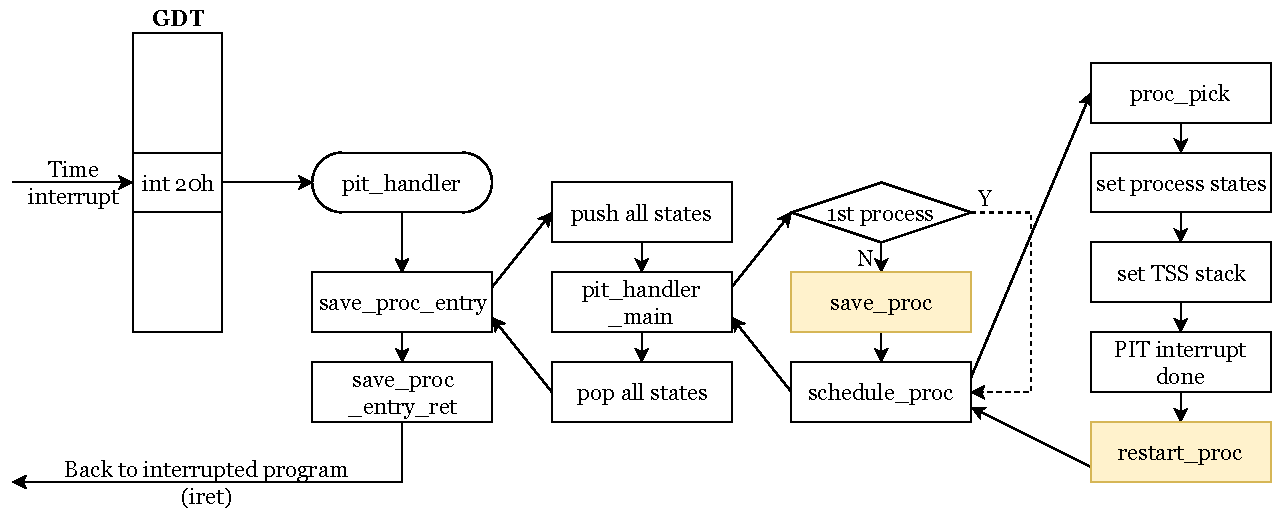
\includegraphics[width=\linewidth]{fig/process-management.pdf}
\caption{进程切换流程图}
\label{fig:process-management}
\end{figure}

当时钟中断到来时,会通过IDT查找到中断处理程序\verb'pit_handler'。
这是一个汇编入口,如下所示。
\begin{lstlisting}[language={[x86masm]Assembler}]
pit_handler:            ; handle process switching
	cli
	jmp save_proc_entry ; DO NOT USE CALL!!! WILL DESTROY STACK
save_proc_entry_ret:
	sti
	iretd
\end{lstlisting}

注意进程切换过程中一定要小心翼翼,如何多余的操作都会导致全局崩溃。
故一进入中断处理程序,先关中断,然后立即跳到\verb'save_proc_entry'保存现场。
之所以不用\verb'call'也是防止堆栈被破坏。

由前面硬件中断和返回一节已知,从用户程序(用户态)转到中断处理程序(内核态)发生了堆栈切换,此时栈顶应该还包含原用户程序栈的信息,这点可以加以利用。
故保护现场的过程如下
\begin{lstlisting}[language={[x86masm]Assembler}]
save_proc_entry:
	pusha ; ax,cx,dx,bx,sp,bp,si,di
	push ds
	push es
	push fs
	push gs

	call pit_handler_main

	pop gs
	pop fs
	pop es
	pop ds
	popa
	jmp save_proc_entry_ret
\end{lstlisting}

经过一系列\verb'push'操作后,栈的内容如下
\begin{center}
\begin{tabular}{r|c|c|}\cline{2-3}
 & ss      & \multirow{5}{*}{int}\\\cline{2-2}
 & esp     & \\\cline{2-2}
 & eflags  & \\\cline{2-2}
 & cs      & \\\cline{2-2}
 & eip     & \\\cline{2-3}
 & eax     & \multirow{8}{*}{pusha}\\\cline{2-2}
 & ecx     & \\\cline{2-2}
 & edx     & \\\cline{2-2}
 & ebx     & \\\cline{2-2}
 & esp     & \\\cline{2-2}
 & ebp     & \\\cline{2-2}
 & esi     & \\\cline{2-2}
 & edi     & \\\cline{2-3}
 & ds      & \multirow{4}{*}{seg}\\\cline{2-2}
 & es      & \\\cline{2-2}
 esp+4 $\to$ & fs      & \\\cline{2-2}
 esp $\to$ & gs      & \\\cline{2-3}
\end{tabular}
\end{center}

由\verb'call pit_handler_main'跳入C函数进行状态保存。
\begin{lstlisting}
void pit_handler_main(
	uint32_t gs,uint32_t fs,uint32_t es,uint32_t ds,
	uint32_t di,uint32_t si,uint32_t bp,uint32_t sp,
	uint32_t bx,uint32_t dx,uint32_t cx,uint32_t ax,
	uint32_t ip,uint32_t cs,uintptr_t flags,
	uint32_t user_esp, uint32_t ss)
{
	// increment tick count
	pit_ticks++;

	if (curr_proc == NULL){
		if (curr_pid != 0)
			schedule_proc(); // no need to save
		interruptdone(0);
		return;
	}

	if (curr_proc->tick > 0){
		curr_proc->tick--;
		interruptdone(0);
		return;
	}

	curr_proc->regImg.eip = ip;
	curr_proc->regImg.cs = cs;
	curr_proc->regImg.eflags = flags;

	curr_proc->regImg.eax = ax;
	curr_proc->regImg.ecx = cx;
	curr_proc->regImg.edx = dx;
	curr_proc->regImg.ebx = bx;

	curr_proc->regImg.esp = sp; 
	curr_proc->regImg.ebp = bp;
	curr_proc->regImg.esi = si;
	curr_proc->regImg.edi = di;

	curr_proc->regImg.ds = ds & 0xFFFF;
	curr_proc->regImg.es = es & 0xFFFF;
	curr_proc->regImg.fs = fs & 0xFFFF;
	curr_proc->regImg.gs = gs & 0xFFFF;

	curr_proc->regImg.ss = ss;
	curr_proc->regImg.user_esp = user_esp;

	schedule_proc(); // change another process

	// tell hal we are done
	interruptdone(0);
}
\end{lstlisting}

注意只有当有进程且要进行进程切换时才进行状态保存,否则都将直接跳过。

这里运用了\textbf{不同特权态下中断处理的堆栈机理}来实现进程的保存,代码十分简洁和清晰。

当一个进程的时间片用完时,就会通过\verb'schedule_proc'函数进行进程调度。
\begin{lstlisting}
void schedule_proc()
{
	process* pp = proc_pick(); // round-robin
	if (pp == NULL) return;
	proc_switch(pp);
}
\end{lstlisting}

这里的\verb'proc_pick'采用最简单的\textbf{轮盘转(round-robin)}方式进行进程的挑选/调度,然后将新的进程送到\verb'proc_switch'中进行进程切换。
\begin{lstlisting}
void proc_switch(process* pp)
{
	if (!(curr_proc == NULL && curr_pid != 0)){
		curr_proc->status = PROC_SLEEP;
	}
	reset_time(pp);

	pp->status = PROC_ACTIVE;
	curr_proc = pp;

	// set up kernel stack
	int stack = 0;
	__asm__ volatile ("mov eax, esp":"=a"(stack)::);
	tss_set_stack(KERNEL_DS,stack);

	interruptdone(0); // IMPORTANT!!!
	restart_proc(
		pp->regImg.gs, pp->regImg.fs, pp->regImg.es, pp->regImg.ds,
		pp->regImg.edi, pp->regImg.esi, pp->regImg.ebp, pp->regImg.esp,
		pp->regImg.ebx, pp->regImg.edx, pp->regImg.ecx, pp->regImg.eax,
		pp->regImg.eip,
		pp->regImg.cs,
		pp->regImg.eflags,
		pp->regImg.user_esp,
		pp->regImg.ss
		);
}
\end{lstlisting}

首先重置新进程的时间片,将其设为活跃进程。

然后设置好TSS段的内核栈---这是保护模式的方便之处,在进程切换过程中可以使用内核栈进行辅助操作,避免复杂的数据移动、指针操作。

在开始恢复现场之前一定要注意告知PIT中断处理已经结束,否则在切入用户态后即使设置了\verb'eflags',也无法使用中断(因为当前中断未结束)。

最后将保存的PCB信息传入\verb'restart_proc',进行现场恢复。
\begin{lstlisting}[language={[x86masm]Assembler}]
restart_proc:
	cli
	add esp, 4   ; skip return address
	pop gs
	pop fs
	pop es
	pop ds
	popa
	iretd        ; flush cs:eip
\end{lstlisting}

理解了堆栈的内容和原理后,其实会发现很简单。
先将栈顶\verb'restart_proc'的返回地址跳过,然后剩下的内容就是我们要恢复的状态了。

由于目前中断处理程序在内核态,而\verb'cs'处在用户态,故\verb'iret'指令\footnote{iretd是32位的返回指令}在执行时先会从TSS中读取内核栈地址\verb'ss0:esp0',作为切换进程的过渡。

跳转到\verb'cs:eip'后,恢复\verb'eflags',然后会将\verb'ss:esp'弹出作为用户栈,最终完成进程切换。

\textbf{整个过程非常简明、流畅,没有多余的东西,既完美地保存了现场,又完美地恢复了现场,成功做到进程切换的无缝连接!}

\subsubsection{多用户程序执行}
在\verb'create_user_proc'中,我创建了四个用户进程,每次创建前都先用IDE将对应硬盘上的程序读入内存,再进行进程创建。
下面是一个例子。
\begin{lstlisting}
read_sectors(ADDR_USER_START,0,2); // addr, sect, cnt
proc_create(USER_CS,USER_DS,ADDR_USER_START);
\end{lstlisting}

注意这里创建的进程都是用户态。
以\verb'cs'为例,除了声明用户态代码段选择子\verb'0x18'外,还需声明请求特权态(requested privilege level, RPL)为3,即ring 3。
将这两者相或得到\verb'0x1b',即为真正的\verb'USER_CS'。
这会在\verb'iret'执行时,实施内核态到用户态的迁移。

完整流程如图\ref{fig:process-run}所示。
\begin{figure}[H]
\centering
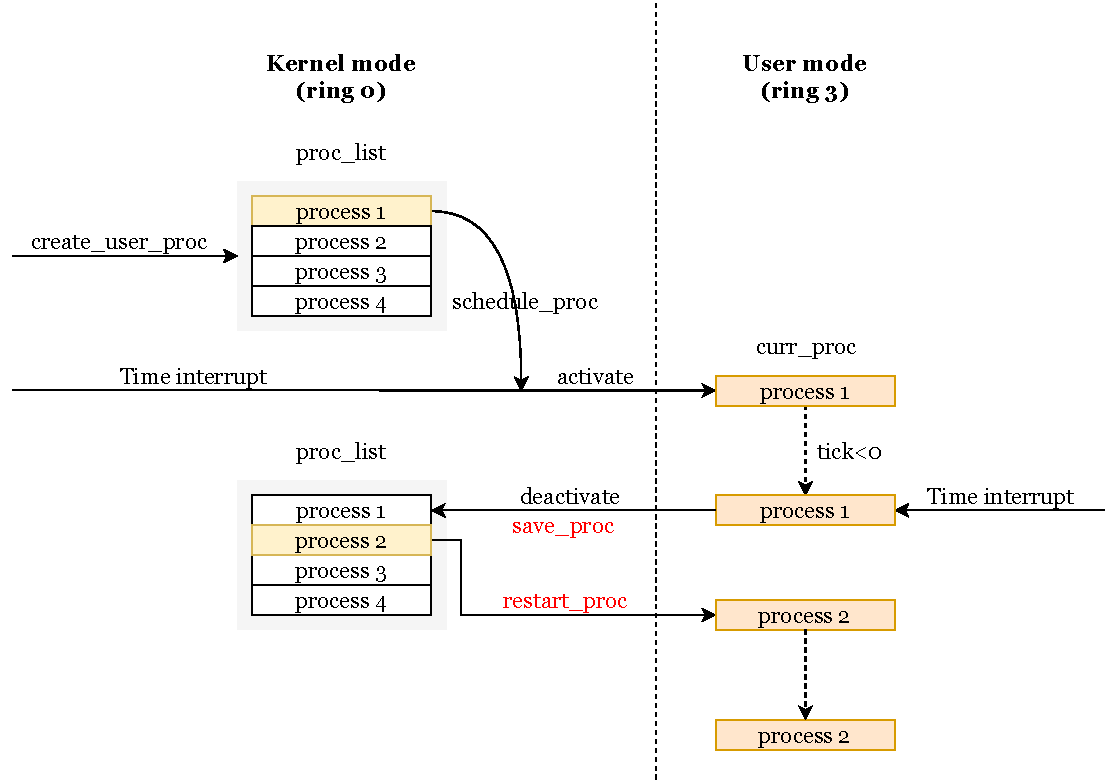
\includegraphics[width=0.8\linewidth]{fig/process-run.pdf}
\caption{进程创建与执行流程图}
\label{fig:process-run}
\end{figure}

\begin{itemize}
	\item Shell中解析到\verb'exec'指令后,调用\verb'create_user_proc'函数
	\item 关中断,创建四个用户进程,然后开中断
	\item 下一个时钟中断来临时,调用\verb'schedule_proc'进行调度(注意现在还在内核态,第一次执行时不会进行进程保存)
	\item 通过\verb'proc_switch'中的\verb'restart_proc'函数,启动第一个进程,由\textbf{内核态切入用户态},且保持中断开启
	\item 在第一个进程执行过程中,遇到时钟中断,\textbf{由用户态切回内核态}进行中断处理
	\item 判断时间片用完,则先进行进程状态保存,然后调用\verb'schedule_proc'切换进程,如此往复
\end{itemize}

\section{实验结果}
\begin{figure}[H]
\centering
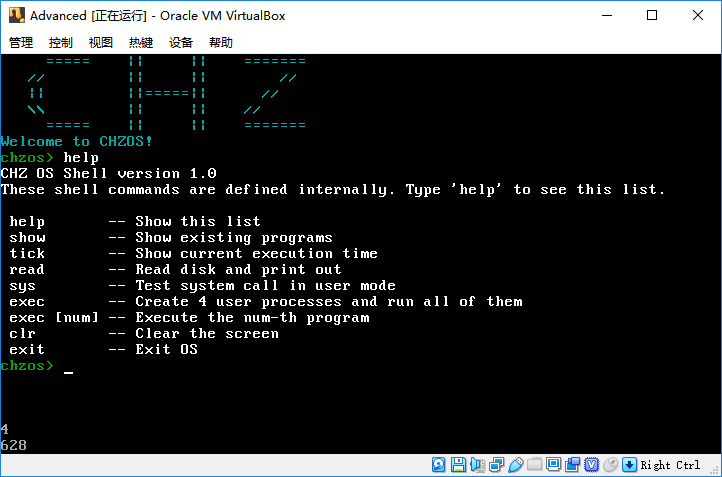
\includegraphics[width=0.8\linewidth]{fig/help.PNG}
\caption{Shell交互界面,左下角显示的是当前运行的时间(0.1s),可以通过设置隐藏}
\end{figure}

\begin{figure}[H]
\centering
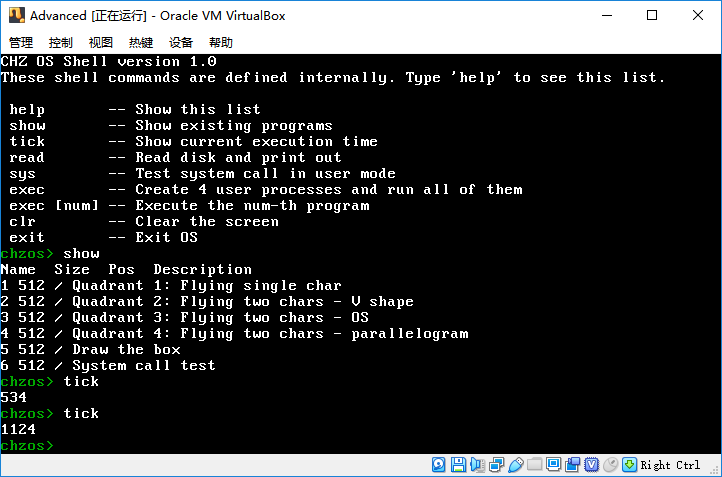
\includegraphics[width=0.8\linewidth]{fig/show.PNG}
\caption{滚屏、时钟计数、用户程序展示测试}
\end{figure}

\begin{figure}[H]
\centering
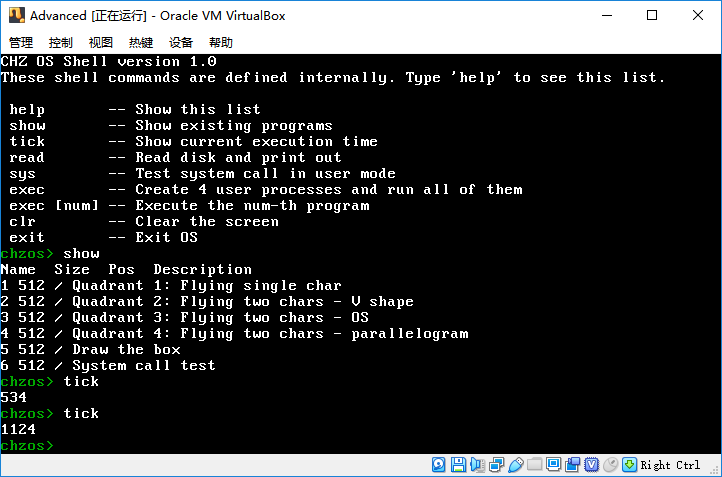
\includegraphics[width=0.8\linewidth]{fig/show.PNG}
\caption{滚屏、时钟计数、用户程序展示测试}
\end{figure}

\begin{figure}[H]
\centering
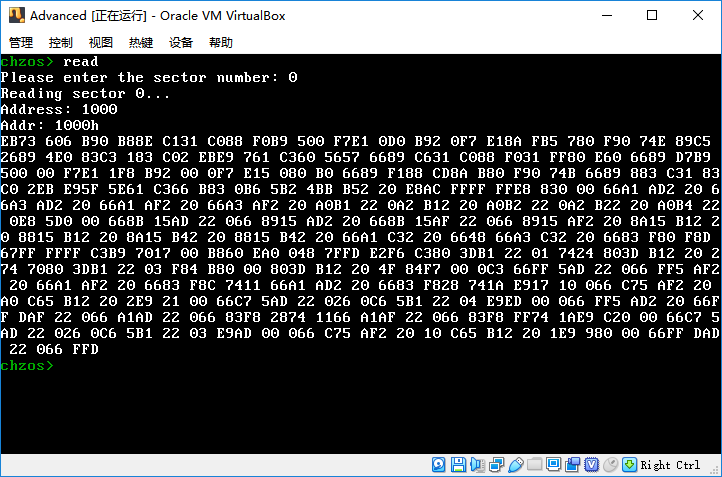
\includegraphics[width=0.8\linewidth]{fig/read_disk.PNG}
\caption{读虚拟硬盘测试}
\end{figure}

C内核中进程表的管理和进程的创建已在前文阐述,设置\verb'MAX_PROCESS'为4即可。
\begin{figure}[H]
\centering
\begin{tabular}{c}
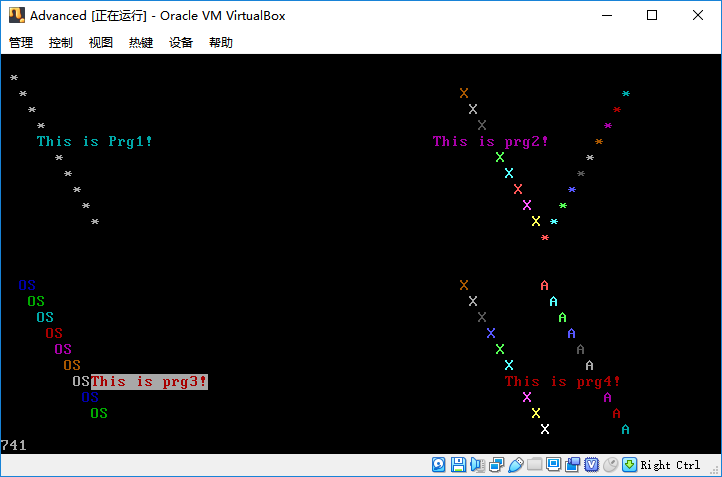
\includegraphics[width=0.8\linewidth]{fig/multi-process-1.PNG}\\
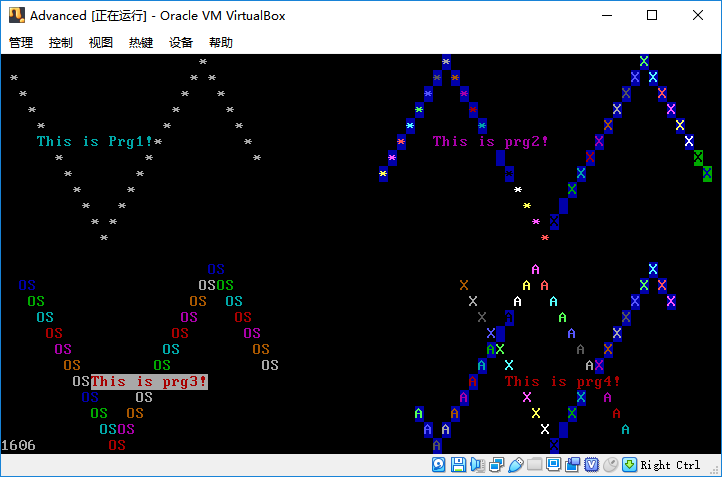
\includegraphics[width=0.8\linewidth]{fig/multi-process-2.PNG}
\end{tabular}
\caption{多进程切换执行,注意\textbf{每个程序的动态变化},从\textbf{左下角的时钟计时}也可以看出这几个进程在同时运行}
\end{figure}

为测试\textbf{用户态ring 3}下的系统调用(\textbf{返回内核态ring 0}),我编写了测试程序\verb'sys_test.asm',如下
\begin{lstlisting}[language={[x86masm]Assembler}]
main:
	mov eax, 0
	int 80h
	mov eax, 1
	int 80h
	jmp $
\end{lstlisting}

对于该测试程序我同样创建了一个进程用于执行。
\begin{lstlisting}
create_one_proc(6); // the 6th program
\end{lstlisting}

测试结果如下图所示,可以看出中断调用正常工作。
\begin{figure}[H]
\centering
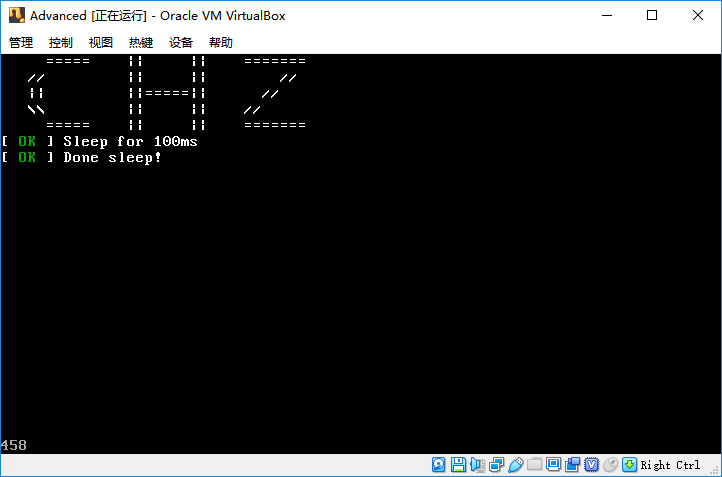
\includegraphics[width=0.8\linewidth]{fig/syscall.PNG}
\caption{系统调用服务正常工作}
\end{figure}

对于未设置特权级别的中断,用户程序是无法调用的,否则会出现如下图所示的保护错误(GF)。
测试样例是在前一个程序的基础上,添加了\verb'int 98h'在\verb'int 80h'后面,以说明\textbf{保护模式真的起到了保护!}
\begin{figure}[H]
\centering
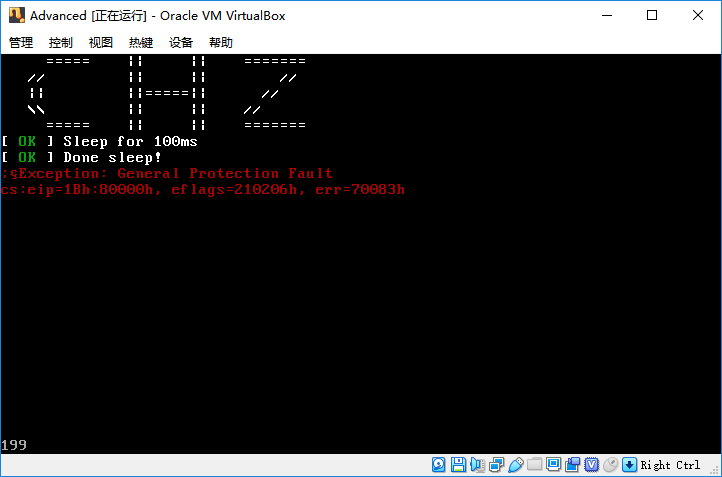
\includegraphics[width=0.8\linewidth]{fig/syscall-GF.PNG}
\caption{测试非系统调用中断0x98出现GF异常}
\end{figure}

\section{实验总结}
% 每人必需写一段,文字不少于500字,可以写心得体会、问题讨论与思考、新的设想、感言总结或提出建议等等。不得抄袭,否则按作弊处理。
本次实验正式进入保护模式,果然如老师所说,保护模式的工程量远远大于实模式的工程量。
一开始不以为意,认为只要在原来实模式的基础上稍作修改即进入保护模式。
但查阅了大量资料之后,发现我错了。
保护模式完全就是一个深不见底的巨坑,大量听都没听说过的名词向你涌来。
保护模式重点就在于保护,所以在CPU中添加了大量基础设施来给予操作系统支持。
各种中断门、调用门、描述符表、任务状态段等等,每一个名词都需要好好理解其深刻含义。

从一开始的茫然无知,到后来了解了保护模式的各种名词含义,再到将这些概念具体实现出来,这其中的艰辛只有我自己知道。
这一个月里,我每天每时每刻都在想着操作系统怎么做,图\ref{fig:web}可以清晰地反映出这一点。
搜索了大量网页和资料,阅读了大量的操作系统源代码,甚至于Intel CPU近5000页的说明书也一页一页啃。
各种资料的叙述方式、实现方式不同,也导致理解上的困难。
有时尝试了多种方法,最终才确定一种真正可行的可以用在我的系统中的实现。
从前文实验步骤看好像保护模式也没什么,但这些都是我经过深刻理解后凝聚出来的结晶啊!
\begin{figure}[H]
\centering
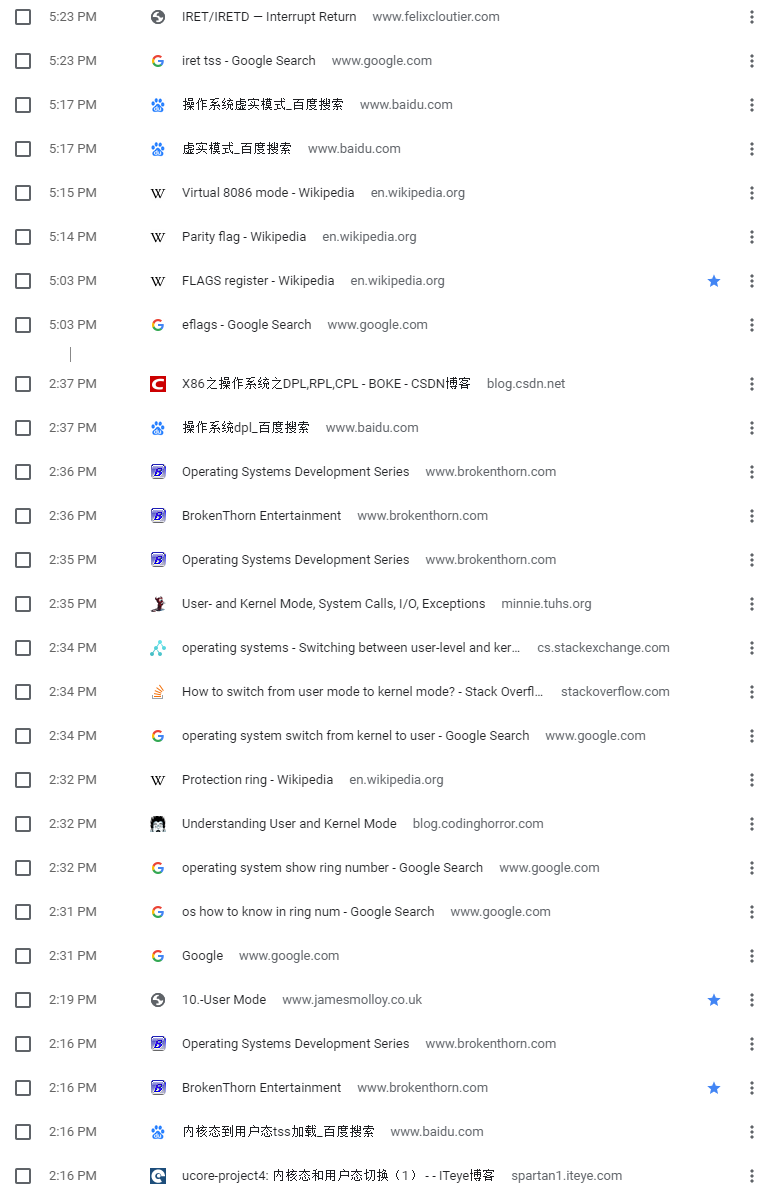
\includegraphics[width=0.6\linewidth]{fig/web-history.PNG}
\caption{网页搜索历史记录}
\label{fig:web}
\end{figure}

操作系统真的是说与做之间存在巨大的鸿沟。
要讲好操作系统中的那些概念很简单,但是要实现得好则非常考编程功底与技艺。
相比起其他上层应用程序,操作系统直接与底层硬件打交道,需要对CPU的工作原理、操作系统中各种概念都理解得非常透彻,才能真正实现出相应的功能。
否则某一条语句没有写,或者某几条语句顺序调换,都会导致系统崩溃。
就如本次实验的进程切换保护和恢复现场是我用Bochs一行一行调试,尝试了上百次才调出来的正确的结果。
一些很细微的错误如果没有注意到,那往往要调上几天都调不出来。

正如前面所说,除了概念非常多,需要理解得很透彻外,操作系统难还难在它难以debug。
操作系统不像上层应用,编译器在编译时会告诉你问题所在。
而现在你是编译器以下系统软件的提供者,这些东西都需要你自己写时,就不再有人给你提供报错信息了。
而且操作系统还具有实时性,出现问题往往难以复原,导致有时会出现bug,有时又不会,总是跟你捉迷藏。
操作系统往往还牵一发而动全身,难以定位问题所在。
有时添加了一个\verb'static inline',都会导致原来跑得好好的代码无法运行。
由于涉及底层硬件,影响的因素非常多,不同的机器/模拟器/虚拟机跑出来的结果还可能不一样,这更是使得调试雪上加霜。
像图\ref{fig:break_down}所示的系统崩溃几乎天天都会出现。
\begin{figure}[H]
\centering
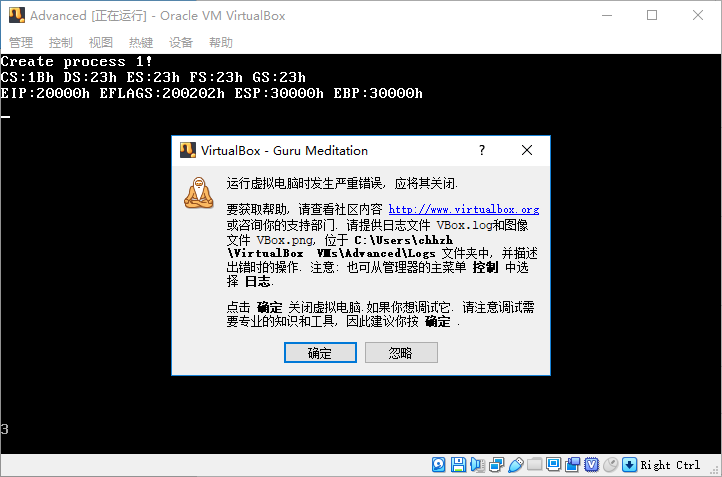
\includegraphics[width=0.8\linewidth]{fig/break_down.PNG}
\caption{系统崩溃}
\label{fig:break_down}
\end{figure}

下面列举出一些重大的问题及相应的解决方案,其中每一点都调试了很长时间。
\begin{itemize}
\item 由于一开始想着新的系统新的环境,故想要升级我的工具。
没想到出师未捷身先死,VirtualBox卸载/安装过程中每每出现蓝屏\verb'DRIVER_IRQL_NOT_LESS_OR_EQUAL',使得卸载/安装无法完成。
最后还是结合自己刚学的操作系统知识,发现是\verb'nwifi.sys'文件出了问题,通过禁用系统WiFi,重新卸载/安装VirtualBox就得以成功。
\item VirtualBox默认参数默认端口未给出,对开发者不友好。
这一点是在编写磁盘驱动时遇到的问题,调试时根本不知道错误是否是由于默认端口号而导致的。
来来回回尝试了几种不同的方案,最终才确定使用IDE/ATA方式读硬盘(主要是因为只有这一种跑得通)。
像Bochs这种,显式通过配置文件指定端口号的,对于操作系统开发就友好很多,但其GUI及模拟速度常常被人诟病。
\item 指针指向的地址与存放指针的地址没有搞清楚,导致程序入口地址传入错误,用户程序无法正常运行。
像在C程序中声明\verb'void* new_addr = (void*)0x20000',若传入汇编的为参数\verb'new_addr',则要注意此时它代表的是一个指针的地址,而不是指针指向的地址。
故保险起见,应该显式地将地址传递入汇编程序中,避免不必要的指针转换。
\item 任务切换堆栈的问题前面已经提到过,卡了好几天,问题极其难以定位,有时用VirtualBox可以运行Bochs又不行,有时用Bochs可以运行VirtualBox又不行。
最终是靠不断在程序中的不同地方加\verb'jmp $'指令使其停止在该位置后,通过Bochs的\verb'print-stack'功能,查看堆栈,然后一行一行debug过来的。
\item 有时为了调试,直接将Shell代码注释掉后将进程读入、创建函数放在程序入口,用VirtualBox运行会直接崩溃,但正常放在Shell中运行都是不会崩溃的(会详细报错)。
查VirtualBox的log发现是\verb'controller not ready for writing',这个问题的答案就呼之欲出了。
由于硬盘还在初始化中,还未准备好,故直接读取硬盘肯定会出问题的。
故解决方案就是在入口处用\verb'sleep'函数先等待一段时间,然后再进行进程创建。
\item 进程状态经过\verb'proc_restart'函数正常恢复后却发现时钟中断无法正常运作,导致下一个进程无法切换。
即使设置了\verb'eflags'的中断标志位\verb'0x200'也还是不行。
这一点跟同学讨论后发现是我在时钟中断处理过程中,先关了中断,但在进用户程序之前没有发送\verb'interrupt(0)'指令告诉外围设备中断已经处理结束,导致新的中断无法正常到来。
\item 单一进程管理全部没有问题后,上多个进程又是不行。
一开始还以为是进程堆栈的问题,于是疯狂在内核中debug。
后来才发现是自己又忘记改用户程序的\verb'org',导致成功加载用户程序后却无法执行。
\end{itemize}

这一个月来经历过多少奇奇怪怪的问题,真的每遇到一个都尝试想要放弃,因为往往一个问题卡上几天是常有的事情。
而且由于操作系统每个人的机器不一样、环境不一样、实现的方式不一样,导致别人的意见、方法都只能作为参考,而不能直接拿来用,真正要解决问题还是要靠自己。
每次都告诉自己要冷静下来,思考问题所在,然后耐下性子来逐行逐行进行调试。

从有想要做保护模式的想法,重新从实验一的内容做起,一直做到实验六,经过快一个月时间,终于终于把保护模式操作系统的原型实现。
耗费了大量精力,完全重构,代码量5356行,最终所有的bug都被我修完,从Github仓库提交记录(见图\ref{fig:github})可以看出这期间我经历了多少艰辛。
\begin{figure}[H]
\centering
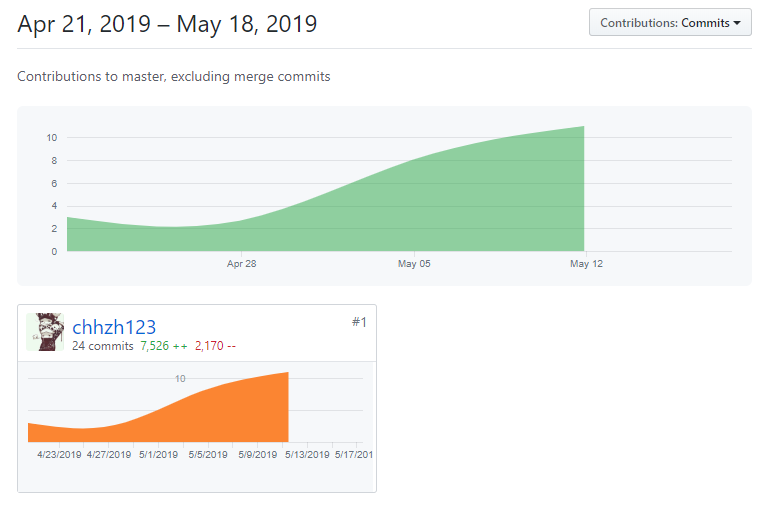
\includegraphics[width=0.8\linewidth]{fig/github.PNG}
\caption{Github提交记录}
\label{fig:github}
\end{figure}

这绝对是一次可以被我铭记终生的系统实现,兴奋之时也要望向前路。
这个学期还没有结束,保护模式操作系统这条路只是一个开端,后续的精彩还等着我继续去探索。


\section{参考资料}
\begin{enumerate}
	\item OS Development Series, \url{http://www.brokenthorn.com/Resources/OSDevIndex.html}
	\item Roll your own toy UNIX-clone OS, \url{http://www.jamesmolloy.co.uk/tutorial_html/}
	\item The little book about OS development, \url{http://littleosbook.github.io/}
	\item Writing a Simple Operating System from Scratch, \url{http://www.cs.bham.ac.uk/~exr/lectures/opsys/10_11/lectures/os-dev.pdf}
	\item Intel$^{\textregistered}$ 64 and IA-32 Architectures Software Developer's Manual
	\item UCore OS Lab, \url{https://github.com/chyyuu/ucore_os_lab}
	\item CMU CS 15-410, Operating System Design and Implementation, \url{https://www.cs.cmu.edu/~410/}
	\item 李忠,王晓波,余洁,《x86汇编语言-从实模式到保护模式》,电子工业出版社,2013
\end{enumerate}

\appendix
\appendixconfig
\section{程序清单}
\subsection{内核核心代码}
\begin{center}
\begin{tabular}{|c|l|l|}\hline
\textbf{序号} & \textbf{文件} & \textbf{描述} \\\hline
1 & \verb'bootloader.asm' & 主引导程序\\\hline
2 & \verb'kernel_entry.asm' & 内核汇编入口程序\\\hline
3 & \verb'kernel.c' & 内核C入口程序\\\hline
4 & \verb'Makefile' & 自动编译指令文件\\\hline
5 & \verb'bootflpy.img' & 引导程序/内核软盘\\\hline
6 & \verb'mydisk.hdd' & 虚拟硬盘\\\hline
7 & \verb'bochsrc.bxrc' & Bochs配置文件\\\hline
\end{tabular}
\end{center}

\subsection{内核头文件}
\begin{center}
\begin{tabular}{|c|l|l|}\hline
\textbf{序号} & \textbf{文件} & \textbf{描述} \\\hline
1 & \verb'disk_load.inc' & BIOS读取磁盘\\\hline
2 & \verb'show.inc' & 常用汇编字符显示\\\hline
3 & \verb'gdt.inc' & 汇编全局描述符表\\\hline
4 & \verb'gdt.h' & C全局描述符表\\\hline
5 & \verb'idt.h' & 中断描述符表\\\hline
6 & \verb'hal.h' & 硬件抽象层\\\hline
6.1 & \verb'pic.h' & 可编程中断控制器\\\hline
6.2 & \verb'pit.h' & 可编程区间计时器\\\hline
6.3 & \verb'keyboard.h' & 键盘处理\\\hline
6.4 & \verb'tss.h' & 任务状态段\\\hline
6.5 & \verb'ide.h' & 硬盘读取\\\hline
7 & \verb'io.h' & I/O编程\\\hline
8 & \verb'exception.h' & 异常处理\\\hline
9 & \verb'syscall.h' & 系统调用\\\hline
10 & \verb'task.h' & 多进程设施\\\hline
11 & \verb'user.h' & 用户程序处理\\\hline
12 & \verb'terminal.h' & Shell\\\hline
13 & \verb'scancode.h' & 扫描码\\\hline
14 & \verb'stdio.h' & 标准输入输出\\\hline
15 & \verb'string.h' & 字符串处理\\\hline
\end{tabular}
\end{center}

\subsection{用户程序}
用户程序都放置在\verb'usr'文件夹中。
\begin{center}
\begin{tabular}{|c|l|l|}\hline
\textbf{序号} & \textbf{文件} & \textbf{描述} \\\hline
1-4 & \verb'prgX.asm' & 飞翔字符用户程序\\\hline
5 & \verb'box.asm' & 画框用户程序\\\hline
6 & \verb'sys_test.asm' & 系统中断测试\\\hline
\end{tabular}
\end{center}

\end{document}

% 实验提交内容
% 实验报告:电子版(Word2003的DOC格式或PDF格式)
% 原程序文件及可执行代码程序文件
% 测试输入数据文件和输出数据文件
% 虚拟机软盘映像文件

% 基础实验项目5个和扩展实验7个
% 实验项目,迟交影响成绩评价!
% 工具与环境可由选择,开发新型工具或优化一套开发环境都可加分!
% 一系列基础实验项目必须连续完成,当前项目只能在前一个项目的基础上进行,体现出前后的进化关系,否则要被约谈,证明没有抄袭行为!
% 一个项目可提交多个改进的版本,实现新功能和个性化特征都有利于提高相应项目的成绩。
% 实验项目提交内容用winrar工具整体压缩打包,统一格式命名为:
%    <学号>+<姓名>+<实验项目号>+<版本号>.rar
%    姓名(学号)实验NvX.zip
%    实验报告、项目文件夹、映像文件
%    ftp://172.18.216.232 sysuac 下周六23:59

% 免考
% 条件:实验1~6全部评价AAAAB+B+或相当
% 最终成绩可能范围:75分以上